%%%%%%%%%%%%%%%%%%%%%%%%%%%%%%%%%%%%%%%%%%%%%%%%%%%%%%%%%%%%%%%%%%%%%%%%%%%
% * <sonya.hanson@choderalab.org> 2015-04-23T18:56:00.248Z:
%
% 
%
% HEADER: DON'T EDIT THIS!
%%%%%%%%%%%%%%%%%%%%%%%%%%%%%%%%%%%%%%%%%%%%%%%%%%%%%%%%%%%%%%%%%%%%%%%%%%%
% ^ <sonya.hanson@choderalab.org> 2015-04-23T18:57:46.938Z.
% But why not?

\documentclass[11pt]{article}

\title{ Advancing predictive physical modeling through focused development of model systems to drive new modeling innovations}

\usepackage[top=0.5in, bottom=0.5in, left=0.5in, right=0.5in]{geometry}
\usepackage{helvet}
\usepackage{url} % hypderref?
\usepackage{graphicx}
\graphicspath{{figures/}} % The figures are in a figures/ subdirectory.
\renewcommand{\familydefault}{\sfdefault}
\pagestyle{empty}
%\pagestyle{plain}
\usepackage{wrapfig}

% Fancy page-width tables
\usepackage{tabularx}

% Use a package for framed boxes
\usepackage{mdframed}

\usepackage[T1]{fontenc}
\usepackage{amssymb}


\usepackage{setspace}
\usepackage{microtype}

\usepackage{amsfonts}
\usepackage{amsmath}

\usepackage{floatrow}

\usepackage[normalem]{ulem} % for nci.bst

\usepackage{sidecap}
\usepackage[abs]{overpic}
\usepackage{wrapfig}

%\usepackage[round,authoryear]{natbib}
\usepackage{cite}
%\setlength{\bibsep}{0.00in}

\usepackage{hyperref}
\hypersetup{colorlinks=true, urlcolor=black, citecolor=black, linkcolor=black}

\newcommand{\doi}[1]{\href{http://dx.doi.org/#1}{doi:#1}}

\newcommand{\ac}[1]{{\sc \lowercase{#1}}}

\renewcommand{\baselinestretch}{.93}
%\renewcommand{\baselinestretch}{.90}
\usepackage{wrapfig} 

\usepackage{bibspacing}
\setlength{\bibspacing}{\baselineskip}


\graphicspath{{figs/}}

\makeatletter

\newcommand{\captionfonts}{\footnotesize}

\makeatletter  % Allow the use of @ in command names
\long\def\@makecaption#1#2{%
  \vskip\abovecaptionskip
  \sbox\@tempboxa{{\captionfonts #1: #2}}%
  \ifdim \wd\@tempboxa >\hsize
    {\captionfonts #1. #2\par}
  \else
    \hbox to\hsize{\hfil\box\@tempboxa\hfil}%
  \fi
  \vskip\belowcaptionskip}      
\makeatother

\renewcommand{\figurename}{{\bf Figure}}

% Page numbering.
%\pagestyle{plain}
%\pagenumbering{arabic}

\setlength{\abovecaptionskip}{-5pt}

\makeatother

\renewcommand{\refname}{Bibliography and References Cited}

\setlength{\parindent}{0pt} % Don't indent first line
%\setlength{\parskip}{1ex plus 0.5ex minus 0.2ex} % Add some space between paragraphs
\setlength{\parskip}{0.8ex} % Add some space between paragraphs

\begin{document}

%======================================
% CITE OUR REFS FIRST
%\phantom{
%\cite{mobley-chodera-dill:2006:jcp:orientation-restraints,mobley-chodera-dill:2007:jctc:confine-and-release,shirts-mobley-chodera-pande:2007:jpcb:dispersion-corrections,chodera:jcp:2007,shirts-mobley-chodera:2007:annu-rep-comput-chem:prime-time,shirts-chodera:jcp:2008:mbar,ncmc,chodera-shirts:jcp:2011:gibbs,chodera:curr-opin-struct-biol:2011:drug-discovery,chodera-shirts:jcamd:2013:yank}
%\cite{gunner:biophys-j:1997:mcce,gunner:bba:2000:proton-electron-transfer,gunner:biophys-j:2002:mcce,gunner:j-comput-chem:2009:mcce2,gunner:jmb:2009:mcce2-hsa,gunner:proteins:2010:reaction-center,dutton:biochem:1994:photosynthetic-reaction-center,gunner:proteins:2010:reaction-center,gunner:photosynth-res:2013:photosynthetic-reaction-center,gunner:bba:2000:proton-electron-transfer,gunner:j-comput-chem:2009:mcce2,nielsen-gunner-garciamoreno:proteins:2011:pka-cooperative,stanton-houk:jctc:2008:benchmarking-pka-prediction}
%}

%%%%%%%%%%%%%%%%%%%%%%%%%%%%%%%%%%%%%%%%%%%%%%%%%%%%%%%%%%%%%%%%%%%%%%%%%%%
% SPECIFIC AIMS
%%%%%%%%%%%%%%%%%%%%%%%%%%%%%%%%%%%%%%%%%%%%%%%%%%%%%%%%%%%%%%%%%%%%%%%%%%%

%{\large \bf SPECIFIC AIMS}

%\eject

%%%%%%%%%%%%%%%%%%%%%%%%%%%%%%%%%%%%%%%%%%%%%%%%%%%%%%%%%%%%%%%%%%%%%%%%%%%
% SIGNIFICANCE
%%%%%%%%%%%%%%%%%%%%%%%%%%%%%%%%%%%%%%%%%%%%%%%%%%%%%%%%%%%%%%%%%%%%%%%%%%%


%NEED TO CAREFULLY CONSIDER GRAPHICS -- SOMETHING ON SIGNIFICANCE?

{\large \bf SIGNIFICANCE}
%2 pages

%Should I be adding boldface mini-summaries here to make it easier to skim?

%Promise of physical methods, how they could transform drug discovery and the design of new small molecules for chemical biology
% (If space permits here we will allude also to how this could help with broader areas too such as engineering of biologics)
Physical methods are poised to transform drug discovery and chemical biology by enabling true molecular design. 
While modeling work is already used extensively in drug discovery, its main role at present is to aid with idea generation or to filter large libraries of compounds for screening. 
Instead, we imagine using computational techniques extensively to guide the design process. 
Consider a medicinal chemist in the not-too-distant future who has just finished synthesizing several new derivatives of an existing inhibitor as potential drug leads targeting a particular biomolecule, and has obtained binding affinity or potency data against the desired biomolecular target. 
Before leaving work, he or she generates ideas for perhaps 100 new compounds which could be synthesized next, then sets a computer to work overnight prioritizing them. 
By morning, the compounds have all been prioritized based on reliable predictions of their affinity for the desired target, selectivity against alternative targets which should be avoided, solubility, and membrane permeability.  
The chemist then looks through the predicted properties for the top few compounds and selects the next ones for synthesis. 
If synthesizing and testing each compound takes several days, this workflow compresses roughly a year's work into a few days.

While this workflow is not yet a reality, huge strides have been made in this direction, with calculated binding affinity predictions now showing real promise~\cite{mobley_perspective_2012, christ_accuracy_2014, deng_distinguishing_2015, sherborne_preprint_2016, schrodinger_accurate_2015, christ_binding_2016, cui_affinity_2016, verras_free_2016}, solubility predictions beginning to come online~\cite{schnieders_structure_2012, park_absolute_2014, liu_using_2016}, and predicted drug resistance/selectivity also apparently tractable~\cite{leonis_contribution_2013}, with some headway apparent on membrane permeability~\cite{lee_permeability_2016, comer_permeability_2014}. 
A considerable amount of science and engineering still remains to make this vision a reality, but, given recent progress, the question now seems more one of \emph{when} rather than \emph{whether}. 

Recent progress in computational power, especially the widespread availability of graphics processing units (GPUs) and advances in automation~\cite{liu_lead_2013} and sampling protocols, have helped simulation-based techniques reach the point where they now appear to have sufficient accuracy to be genuinely useful in guiding pharmaceutical drug discovery at least for a certain subset of problems~\cite{mikulskis_large-scale_2014, homeyer_binding_2014, sherborne_preprint_2016,  schrodinger_accurate_2015, christ_binding_2016, cui_affinity_2016, verras_free_2016}.
Specifically, in some situations, free energy calculations appear to be capable of achieving RMS errors in the 1-2 kcal/mol range with current force fields, even in prospective applications.
As a consequence, pharmaceutical companies are beginning to use these methods in discovery projects.

%Limitations of methods and of retrospective tests or application for methods improvements
Unfortunately, these methods still have severe limitations, and a great deal of science and engineering is still needed before these techniques can achieve the major design impact we desire. 
For example, even ``small'' protein conformational conformational changes can yield errors up to 5 kcal/mol in calculated binding free energies~\cite{lim_sensitivity_2016}, and force field limitations can pose major challenges as well~\cite{rocklin_blind_2013}. 
Worse, the most important sources of error are not always clear.

Unfortunately, neither retrospective tests nor application of these techniques in drug discovery provides the necessary impetus and data to rapidly advance physical modeling techniques.
While large-scale retrospective tests can be valuable for assessing how well we can currently do \emph{retrospectively}, they are of limited value for paving the way forward or for assessing how well we will do for molecular design.
Partly, retrospective tests allow for unintentional cheating, where a well-meaning researcher might apply a protocol they know will work in this particular situation where application in a design setting would lead to a different choice of protocol.
For example, if the binding mode of a ligand is already known crystallographically, a researcher may use that binding mode in retrospective tests, whereas prospective or design work would require also selecting candidate binding modes, introducing substantial additional uncertainty~\cite{mobley_predicting_2007, boyce_predicting_2009, mobley_perspective_2012}.
This also means that in retrospective tests, researchers almost invariably try far fewer methods than in prospective tests, resulting in much less new insight.
Prospective application, while important, also does not provide the necessary impetus, partly because often, the predicted compounds are in fact never tested~\cite{christ_binding_2016} or the experimental data necessary to assess the quality of the predictions is absent -- for example, because binding affinities are not measured or no crystallography is available. 

%Explain need for blind challenges and how D3R only fills part of need
To rapidly advance these methods, we need a series of community blind prediction challenges focused specifically on pushing the limits of predictive techniques, beginning from problems which are just barely tractable with today's methods and advancing to problems just past the frontier.
These challenges should be designed to have precisely the necessary high quality experimental data, but also be prospective, predictive tests.
While the Drug Design Data Resource (D3R~\cite{gathiaka_d3r_2016}, discussed further below) provides an existing community blind challenge on protein-ligand binding, it focuses on using \emph{existing} pharmaceutical datasets for blind challenges, and not on introducing new data in a carefully controlled manner in order to maximize the learning value to the community~\cite{gathiaka_d3r_2016}. 
In other words, D3R serves well to assess where we are now -- but we need a carefully designed effort that will help the field achieve our goals.

%Discuss importance of SAMPL (including publication/citation count, previous successes in advancing the field, focus), need for funding to:
%   a. Continue SAMPL
%   b. Allow for "design" of SAMPL (rather than having it be driven by data availability)
%   b. Extend SAMPL to bridge to D3R rather than leaving a "capability gap" (here's where I explain why this is distinct from D3R -- this is crucial)
One series of blind challenges, called ``Statistical Assessment of Modeling of Proteins and Ligands`` (SAMPL) provides a model we carry forward and extend here. 
SAMPL was begun by OpenEye software in 2007/2008~\cite{nicholls_predicting_2008} at one of their CUP science events, and has run approximately every two years since then~\cite{nicholls_samp1_2009, mobley_predictions_2009, geballe_sampl2_2010, geballe_sampl3_2012, mobley_blind_2014-1, muddana_sampl4_2014, bannan_blind_2016, yin_sampl5_preprint}; it transitioned to being run by an outside group of academics beginning partially with SAMPL3 in 2012, then completely for SAMPL4 (2014) and SAMPL5 (2016), with the PI of this proposal playing a key organizational role in SAMPL3-SAMPL5.
SAMPL is modeled as a \emph{challenge} rather than a \emph{competition}, with a key goal being to maximize what is learned rather than to declare winners and losers, with the idea that learning will provide the greatest long-term rewards in terms of progress in the field.
SAMPL has always involved a component focused on calculation of relatively straightforward physical properties such as hydration free energies, but also introduced host-guest systems as model binding systems for SAMPL3-5, supplementing protein-ligand challenges (on trypsin and HIV integrase) which appeared in SAMPL3-4. 
SAMPL has already been a tremendous resource for the community, resulting in roughly 100 publications (some are coming out as of this writing) which are typically cited 5-50 times or more each [refs].
%Add full list of references here.

Here, we continue the legacy of SAMPL, but design a new series of SAMPL challenges specifically to maximize learning value to the community.
Until now, this has been impossible, because SAMPL has been entirely unfunded, so its existence has required ``donation'' of data from various sources rather than data collected specifically to drive improvements to modeling. 
Funding of SAMPL will also allow SAMPL to deliberately bridge the gap between calculations of simple physical properties like hydration -- which can be calculated fairly accurately with today's methods~\cite{mobley_blind_2014-1} -- 
and the D3R Grand Challenges on protein-ligand binding, which are a major source of consternation for the community so far~\cite{ignjatovic_binding-affinity_2016, deng_large_2016, sunseri_d3r_2016, gathiaka_d3r_2016}.
Unless this gap is bridged, there is the very real possibility that modeling may simply continue to fall far short of expectations in pharmaceutical challenges like D3R for reasons which are unclear.
The extension of SAMPL proposed here will allow us to form blind challenges designed to highlight major reasons for failure and drive progress towards resolving them.

%Wrap up with how this will realistically help advance binding prediction in a realistic timeframe (a brief mention of CASP will likely be appropriate even though we don't follow the same model)
Our major goal is to rapidly advance predictive modeling to where it can guide experimental work doing biomolecular design, and extension of the SAMPL challenges will do exactly that.
The Computer Aided Structure Prediction (CASP) series of competitions provide an example of how a focused effort can realistically have a dramatic impact on predictive modeling in a relatively short space of time.  {\bf [JDC to write text here]}
%JDC to write some text on CASP
While our model for the SAMPL challenges is slightly different than that for CASP (for example, we have less emphasis on competition) we see SAMPL playing the same key role in driving predictive modeling, but in our field of protein-ligand interactions. 
In our view it will play a vital role in enhancing the work being done on \emph{existing} data by D3R. 



{\large \bf INNOVATION}
% 1 page

%SAMPL drives science in our groups and in the field
   %a. Give examples from our groups from prior SAMPLs
   %b. Examples from field in prior SAMPLs
Blind predictive challenges -- and SAMPL in particular -- already play a key role in fostering innovation in the field, especially in the form of method development, testing, and hardening, as well as force field development. 
Thus, this work, by continuing and extending SAMPL, will advance innovative new science. 
It is worth briefly highlighting several historical examples, though far more are available in the SAMPL literature. 
The first several SAMPL challenges on hydration free energies had rather hit-and-miss performance, highlighting pitfalls of existing methods and force fields which led to marked improvements in PB models [refs],
%cite OpenEye work
 recognition of some limitations of fixed-charge force fields [refs],
% Hydroxyl stuff we did, also Cerutti
repair of some of these force field deficiencies via additional polarization or introduction of off-site charges [refs],
%Hydroxyl/cerutti/Fennell
and helped motivate alternate implicit or hybrid solvent models [ref].
Together these advances led to a marked improvement in accuracy for calculations of hydration free energies between SAMPLX and SAMPLY (Figure []).
%FILL IN DETAILS ON LINE ABOVE
%
%Add some sort of a figure on how SAMPL has helped community -- maybe compare accuracy in hydration free energies (simple?!?) in an early SAMPL with accuracy on log D in this SAMPL or something similar? Show something that demonstrates progress.
%b.1 Figure showing progression in hydration free energy accuracy across a couple of SAMPLs or comparing two SAMPLs?
%
 %Fennell SEA, etc.
Shifts in protonation state and tautomer proved particularly important in the recent SAMPL5 $\log D$ challenge[refs], as they presumably will be for protein-ligand binding as well.
Host-guest binding studies have also been particularly important[ref benchmark sets],
%reference the benchmark sets paper
highlighting the importance of salt effects [refs]
%Gilson work, other (see cites in benchmark sets)
and in some cases revealing more severe force field limitations than observed in hydration and distribution challenges [ref Gilson group stuff],
%Add ref.
pointing the way forward for improving predictive models of molecular interactions [ref].
%Add something from Gilson group on using this data to improve FFs; also ref benchmark sets paper


%c. Mention uniqueness of SAMPL -- there are other predictive challenges (D3R, pKa coop, CASP) but none focused on driving quantitatively predictive protein-ligand modeling
This work is also innovative because of the uniqueness of SAMPL.
While there are other predictive challenges in the area of biomolecular modeling, such as D3R [ref], the pKa cooperative [ref], and CASP [ref],
%insert references
none are specifically focused on driving quantitatively predictive protein-ligand modeling.
SAMPL is unique because -- at least with the deliberate design plan we propose here -- it will be specifically tailored in order to drive improvements in modeling for biomolecular design.
It also plays an enabling role for a wide variety of other science, rather than functioning as a stand-alone entity. 
SAMPL benefits the whole modeling community -- for example, even docking software has improved from SAMPL hydration challenges [ref Coleman], and even commercial software has introduced new features and made improvements based on SAMPL challenges [cite Klamt stuff].
%Add refs. 
In effect, SAMPL serves as an innovation engine, and this work will ensure that SAMPL not only continues but becomes even more valuable to the community.
 

% Innovation in experimental pipelines (Aim 3)
This work also focuses on innovative experimental methods.
Specifically, in Aim 3, we are developing new, high-throughput experiments for studying and measuring protein ligand binding, with careful automated error analysis, and a heavy emphasis on robotics and automation.
The Chodera lab -- responsible for Aim 3 -- already has substantial expertise in the area of automation of experiments and better uncertainty analysis of those experiments. 
Additionally, they design their own 3D printed parts to facilitate these experiments, and make plans for these available to others. 
Thus this work is at the forefront of innovation in high-throughput, automated experiments to produce high quality data with well characterized uncertainties. 
Not only will the data itself be of prime importance to the community, but the techniques themselves will help future experimental work.
%Add some cites here

% Innovative reference calculations (Aim 4)
In Aim 4, we will not only run SAMPL community challenges, but also perform our own reference calculations with the latest techniques, testing their accuracy and using these to assess the current state-of-the-art.
Both the Mobley and Chodera labs are experts in development of free energy methods for application to physical properties (e.g.. [ a couple refs]) and binding (e.g. [a couple refs]), and the reference calculations we perform in Aim 4 are particularly important for innovation as well, serving several key roles: (1) Benchmarking our latest method developments against current ``best practices'' methods (by doing calculations via both approaches); (2) Facilitating learning, allowing others to experiment with how a change in method or force field impacts results; (3) Focusing the field on key issues by doing sensitivity analysis to whether conditions such as ionic strength, protonation state, tautomer choice, etc. impact computed values.
%Add references

% Innovation in analysis of method performance, comparison of methods, workflow science? (Aim 4)
Innovation in Aim 4 extends beyond reference calculations to analysis of the challenge itself.
When methods differ in performance, it is critical to understand whether the differences are statistically significant and important, and to provide an accurate accounting of the uncertainty in performance measures. 
Thus, careful and innovative analysis of challenge outcomes is particularly important in SAMPL [refs], in some cases driving experimentation with new performance metrics [refs].
%References
Additionally, we try to draw attention to and promote analysis of model uncertainty (as distinct from statistical uncertainty) in calculated values [refs], as understanding the confidence levels of predictions is particularly important for guiding molecular design.
%Cite model uncertainty stuff.


{\large \bf APPROACH}
% 9 pages

Our approach to systematically advancing modeling for biomolecular design involves collecting carefully tailored experimental data for challenges focusing on physical property prediction, host-guest binding, and biomolecular binding.
Thus, we have four main aims, three of which focus on tailoring and generating this experimental data, and a fourth which focuses on running SAMPL challenges to advance modeling and maximize the learning value to the community.
These SAMPL challenges will run yearly (though not necessarily every aspect of the proposal will feature in every SAMPL challenge), so each of the aims focused on generating experimental data has a series of stages which correspond to individual future SAMPL challenges.

%Aim 1 - Generate new data for simple SAMPL blind challenges on physical property prediction (1.5 pages)
{\bf Aim 1: Generate new data for ``simple'' SAMPL blind challenges on physical property prediction.}
%We will develop new solution-phase datasets for druglike small molecules. These data can test critical aspects of small molecule modeling (including accounting for interactions and treatment of protonation/tautomeric state) and improve our ability to predict physical properties relevant to drug discovery in new regions of chemical space. We will initially focus on distribution between organic phases and on pKa's and their modulation by solvent environment, using these data to drive improvements in the modeling of ligand interactions.
Our first aim focuses on generating solution-phase physical property data for small, drug-like molecules -- essentially continuing the tradition begun with hydration free energies in SAMPL0-4 and continued with water-cyclohexane distribution coefficients in SAMPL5. 
Distribution coefficients proved tremendously valuable to the community in SAMPL5 for a number of reasons, highlighting a number of key issues where modeling needs to improve, so they will form the basis for the physical property component in SAMPL6 and return in several subsequent SAMPL challenges.

%Compare log D accuracy vs hydration accuracy, highlight issues and explain relevance to drug discovery; note lessons learned in SAMPL5
     %Maybe use a figure on log D accuracy?
Distribution coefficients proved to be precisely the right level of difficulty for a SAMPL challenge focused on maximizing learning. 
Specifically, they were challenging enough that many methods performed poorly, with even the best methods having accuracies less than would have been expected based on their ability to calculate hydration free energies in water~\cite{bannan_calculating_2016}. 
At the same time, methods typically did well enough that it was possible to learn a great deal from examining failure, and the major sources of error were issues which will also plague prediction of ligand-receptor interactions.
These included neglect of changes in protonation state on transfer between environments, uncertainty as to the relevant protonation state and/or tautomer in one or both environments~\cite{bannan_calculating_2016}, problems with sampling the conformation of some of the larger ligands~\cite{bannan_calculating_2016, luchko_sampl5:_2016}, and force field limitations~\cite{paranahewage_predicting_2016}. 
Our partnership with Genentech for these measurements also meant that the compounds were from Genentech's library and thus very drug-like, unlike typical compounds seen in hydration free energy challenges of the past.
In some respects, distribution coefficients posed the ideal SAMPL challenge, hitting the sweet spot in terms of difficulty -- difficult enough that clear failures were frequent and there is much room for improvement, but not so difficult that the reasons for failure were unclear in general. 
Still, the challenge could have been improved by follow-up experiments to re-check some of the experimental results~\cite{paranahewage_predicting_2016, klamt_prediction_2016, bannan_blind_2016, rustenburg_measuring_2016} -- but without funding for someone to continue working in this space, this has so far been impossible.

%Explain what science -- log D/logP, pKa primarily but mention possible other areas of interest
Because distribution coefficients were so valuable in SAMPL5 and are driving so much needed method development [refs],
%Cite examples of people trying things from SAMPL5
we will measure new cyclohexane-water distribution coefficients for our first data set here and this will form the basis for the physical property component of SAMPL6. 
Because octanol-water distribution coefficients are also potentially tractable~\cite{bannan_calculating_2016}, and measured much more frequently experimentally, we plan to generate measurements for the same compound distributing between both cyclohexane-water and octanol-water for this challenge.

However, distribution coefficients conflate several issues which are still complex, namely protonation state and tautomer prediction, as well as transfer into different environments. 
Thus, we will likely need to turn to separating these issues to improve our handling of them one at a time. 
For SAMPL7, then, our tentative plan is to measure pKa values for an extensive set of drug-like molecules in water and 
%can we also do other solvent(s)?
provide data specifically on pKa values, thereby separating the issues of predicting protonation state from those of transfer.

In the next challenge, SAMPL8, we would re-combine the pKa and transfer issues in a way to maximize learning -- specifically, we will not only measure distribution coefficients but also measure pKa values for the same set of compounds, allowing participants to (a) predict distribution; (b) predict pKa; and (c) predict partitioning.

Several other avenues are of interest for future datasets as well.
New computational techniques are targeting membrane permeability~\cite{lee_permeability_2016, comer_permeability_2014}, and this is experimentally accessible (see support letters from Pfizer and Merck), leading to potential interest in new datasets and challenges focused there.
Alternatively, partition/distribution into other environments aside from cyclohexane or octanol may provide significant value, especially given dielectric constant issues posed by current force fields [ref].
%cite something by Fennell here
%Also mention solubility -- Sirius T3 can measure (though expts aqueous) so that could be intresting.
%Coupounds just need titratable group
  
 %Industry partnerships (and past precedent)
Here, our experimental work will be performed with partners in the pharmaceutical industry, following roughly the model used for SAMPL5, where we partnered with Genentech, sending Bas Rustenburg, a graduate student in the Chodera lab, to conduct measurements of $\log D$ using existing equipment.
We find that pharma often has substantial access to equipment -- such as the expensive Sirius T3 for measuring partition, distribution, and pKa -- which is very hard to find in academia, and it may not always see heavy use. 
Thus, sending a person into pharma to generate data can be an extremely fruitful line of inquiry, as the relevant equipment and expertise is already present but manpower is lacking.
Here, we are partnering with Genentech, Pfizer, and Merck (see support letters), who have agreed to give us access to the equipment and expertise we need for the necessary measurements.
% add GSK if their letter comes in
This work will provide funding for us to send a joint experiment and modeling student from the Mobley group to conduct the relevant measurements with our pharma partners. 
As noted, we already know that this model will work given our experience in SAMPL5~\cite{rustenburg_measuring_2016}, and our pharma partners see the value of this data and the SAMPL challenge to the modeling community.

%Talk about limitations of approach -- lack of ability to do follow up expeirments, get the dynamic range we wanted, test things again after SAMPL? 
% Sustained funding will allow us to do that. 
% (This will also help answer the argument that we don't need funding for this...)




%Aim 2 - Measure binding of novel host-guest complexes for introductory ligand binding challenges (2 pages)
{\bf Aim 2: Measure binding of novel host-guest complexes for introductory ligand binding challenges.}
We will measure new host-guest binding free energies for cucurbiturils and deep-cavity cavitands, yielding further host-guest binding challenges which span between physical property prediction and protein-ligand binding. Host guest systems are some of the simplest cases of molecular recognition, and thus these binding data will drive improvements in modeling of simple binding systems with techniques of relevance to drug discovery.

\begin{center}
{\bf Cucubituril-based receptors as model binding systems}
\end{center}

%Intro lessons learned on HG systems, relevance to drug discovery
%Isaacs science

%Edit to be consistent with Gibb section below -- this uses 3rd person initially.
{\bf Cucubituril derivatives for host-guest binding.} 
The Isaacs group has previously participated in the SAMPL challenges and supplied unpublished host-guest binding constants~\cite{ma_acyclic_2012-2, cao_absolute_2014, She_she_glycoluril-derived_2016}.  
Our participation was quite stimulating for us and influenced our investigation of the biomedical applications of acyclic CB[n]-type receptors (a.k.a Calabadions). 
Cucurbit[n]uril receptors are particularly well suited for the SAMPL challenges because they exhibit: 1) high binding constants toward suitable guests in water (routinely $\mu$M to nM; occasionally pM to fM)~\cite{cao_attomolar_2014, liu_cucurbituril_2005, mock_structure_1986, assaf_cucurbiturils:_2015, moghaddam_new_2011, shetty_can_2015, biedermann_release_2012}, 2) high selectivities between structurally related guests which translate into large $\Delta \Delta G$ values~\cite{isaacs_stimuli_2014}, 3) low molecular weights (1000-2000 amu) which allows high levels of theory to be used, and 4) limited conformational degrees of freedom.  
Herein, we propose to continue to participate in the next three SAMPL challenges during the proposed five year funding period by resynthesizing previously published CB[n]-type receptors of increasing complexity, measure Ka values and determine host-guest stoichiometry and geometry toward biologically relevant guests which will allow the computational chemists to push the boundaries of the free-energy prediction of receptor-igand complexes.  
Figure~\ref{figure:CB} shows the chemical structures of three hosts -- Me4CB[8]~\cite{vinciguerra_synthesis_2015}, glycoluril hexamer~\cite{lucas_templated_2011}, and acyclic CB[n]-type receptors~\cite{ma_acyclic_2012, ma_acyclic_2012-1, zhang_acyclic_2014, gilberg_acyclic_2015, sigwalt_acyclic_2016, zhang_acyclic_2014-1} which span the range from preorganized macrocyclic host to uncharged acyclic but preorganized host to highly charged acyclic host.

\begin{figure}[h]
\begin{centering}
\resizebox{\textwidth}{!}{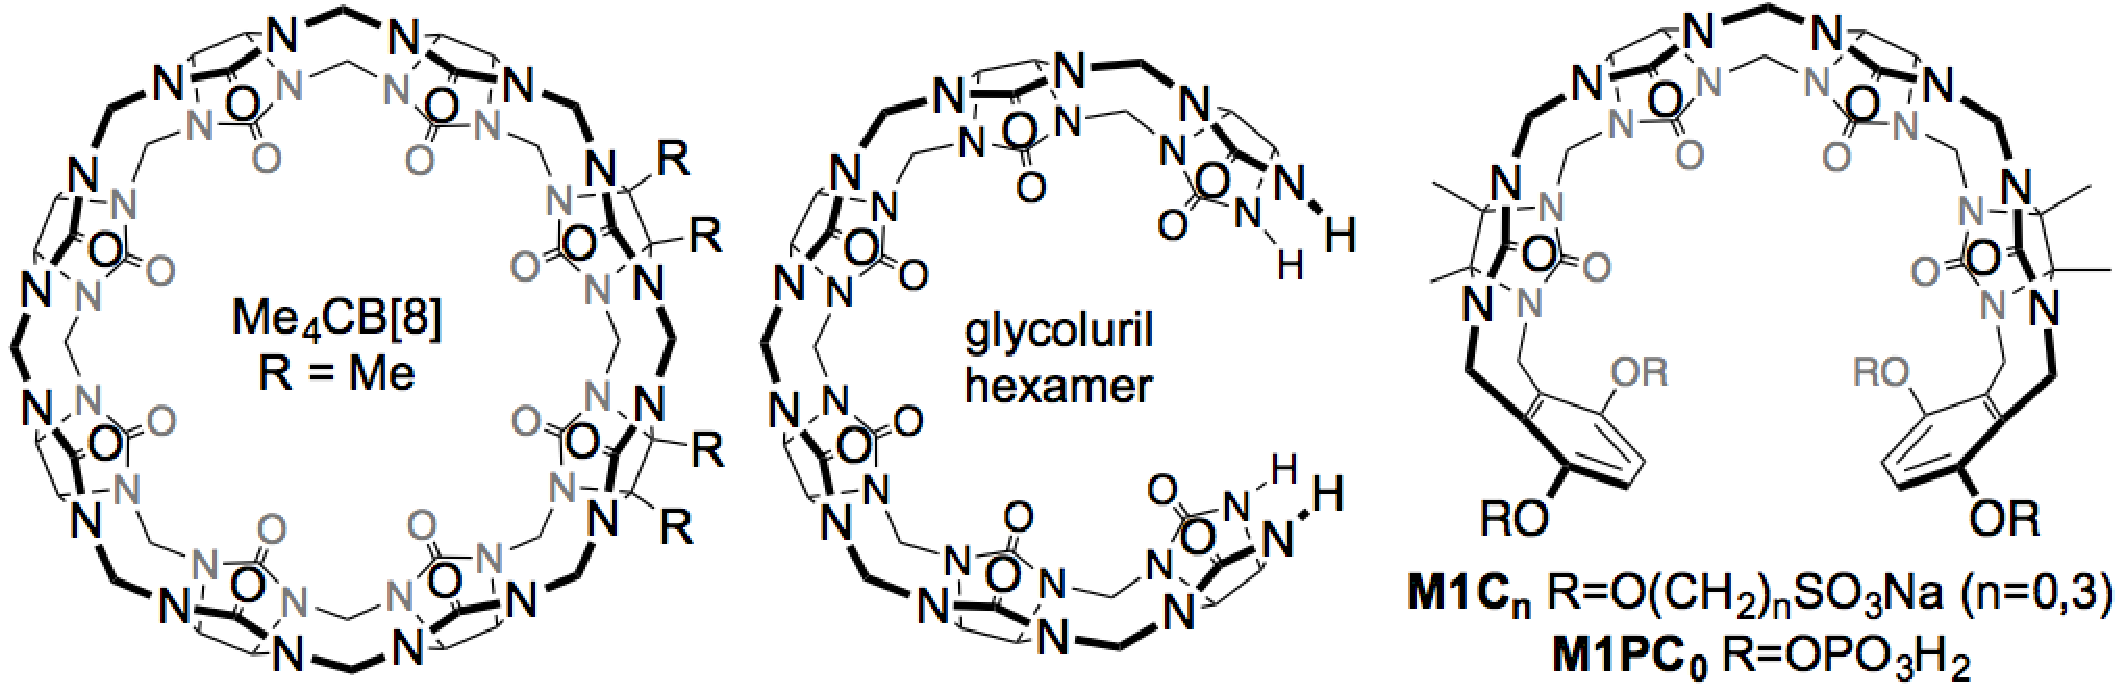
\includegraphics{figures/CB.pdf}}

%\end{centering}
\vspace{0.1in}
\caption{\footnotesize {\bf Structures of Me$_4$CB[8], glycouril hexamer, and acyclic CB[n]-type receptors.}
\label{figure:CB}}
\end{centering}
\end{figure}

\emph{SAMPL6.}  
For this challenge we propose to measure $K_a$ and $\Delta H$ values, stoichiometry, and geometry for the interaction of Me4CB[8] (nicely water soluble CB[8] derivative) toward 15 guests (chosen from top selling drugs, Table CB1) by either direct or competition isothermal titration calorimetry (ITC), UV/Vis or fluorescence indicator displacement assay, or NMR competition experiments which we are very experienced with~\cite{cao_attomolar_2014, liu_cucurbituril_2005, ma_acyclic_2010, she_glycoluril-derived_2016}.  
Our selection of Me$_4$CB[8] and top 100 drugs was based on a desire to increase the level of complexity of the computational challenge by: 1) changing host flexibility (e.g. Me$_4$CB[8] can exhibit ellipsoidal deformation)~\cite{vinciguerra_synthesis_2015}, 2) by allowing the possibility of binary or ternary (e.g. 1:1 and/or 1:2 host:guest) complexes~\cite{ko_supramolecular_2007, barrow_cucurbituril-based_2015, urbach_molecular_2011}, 3) using drugs with several potential binding epitopes to include sampling issues.  Host:guest stoichiometry and geometry (e.g. which binding epitope is complexed) will be addressed by ITC ``n'' values, Job plots monitored by UV/Vis or NMR~\cite{connors_binding_1987}, and by 1H NMR complexation induced changes in chemical shifts~\cite{masson_cucurbituril_2012}.  
All three sets of studies will be conducted in phosphate buffered saline (pH 7.4 with physiological salt) which introduces further complexity due to competitive interaction between the C=O portals of CB[n]-type receptors and metal ions via ion-dipole interactions which reduces the observed Ka values~\cite{marquez_mechanism_2004}.

\begin{wraptable}{l}{7.5cm}
\begin{tabular}{l | l}
{\bf drug} & {\bf features} \\
\hline
memantine & adamantane; 1:1 \\
saxagliptin & adamantane; 1:1 \\
premarin & steroid \\
pancuronium & steroid\\
varenicline & 1:1 vs 1:2 \\
valsartan & pKa 4.37 \\ 
omeprazole & pKa 4.77 \\
ranolazine & pKa 7.17; epitopes \\
pradaxa & pKa 3.87; epitopes \\
nilotinib & epitopes; pKa 6.3 \\
sensipar & epitopes; folding \\
vyvance & diamine; epitopes; folding \\
minocycline & tetracyclin; amino aniline \\
\end{tabular}
\caption{\label{table:CB} Selected drugs as guests }
\end{wraptable}

\emph{SAMPL8.} 
We propose to study host:guest complexes of glycoluril hexamer toward the 15 drugs (Figure CB1).  
We select glycoluril hexamer for this challenge because it: 1) increases the conformational dynamics of the host, and 2) influences the number and energy of solvating (and unusually coordinated) water molecules that are implicated in the observed high binding constants for CB[n]-guest complexes~\cite{biedermann_release_2012, biedermann_hydrophobic_2014}.  
Furthermore, in selecting the drugs, we have chosen several that have pKa values in the 3.8 to 7.4 range.  
Similar to biomolecular host-guest systems, CB[n]-type receptors are well known to induce pKa shifts (up to 4 pKa units) of complexed guests~\cite{saleh_activation_2008, nau_deep_2011, ghosh_strategic_2012}, and the ability of computation to replicate and predict such shifts and their impact on Ka are of high significance.
 
\emph{SAMPL10.} 
We will focus on acyclic CB[n]-type receptors (e.g. M1C$_3$, M1C$_0$, and M1PC$_0$ that contain anionic solubilizing groups attached via different linker lengths.  
As in SAMPL2, these acyclic CB[n]-type receptor introduces conformational complexity and influences the free energy of the solvating H$_2$O molecules in the free host.  
Moreover, the presence of 4 anionic groups in close proximity to the cavity are expected to have a significant influence on the balance between ion-dipole interactions and the solvation of the free host.



\begin{center}
{\bf Gibb deep cavity cavitands for host-guest studies} 
\end{center}

%Gibb science

%CHODERA FEEDBACK TO INCORPORATE HERE:
%* We need to emphasize why the octa-acid system has proven to be so valuable for modelers in the introduction: What specific physical challenges does the system probe, and what have we learned? We also need to add citations to the meta-analysis and maybe even all of the papers that addressed this system. David can likely address this.
%* I'm a bit concerned that proposing to measure only five ligands per compound is going to be perceived as lacking in statistical power required to assess accuracy, and that this specific aspect will be a liability. Is it possible to do more than that, or would this require a significantly larger chunk of money or access to automated ITC technology? Alternatively, we can be vague about how many compounds we will use or focus on the total number of compounds across all hosts. (DLM: I should probably recast a bit somewhere to explain how much we'll learn across hosts.)

{\bf History of octa-acid SAMPL challenges.} During SAMPL4~\cite{gibb_binding_2013} and SAMPL5~\cite{sullivan_binding_2016} we focused on two hosts: the octa-acid 1 (R = H) and another octa-acid derivative with four methyl groups positioned at the portal of the binding pocket (1, R = Me). 
% Chodera suggests commenting on what specific features of these hosts were remarkable for presenting isolated challenges to quantitative predictive modeling -- sterics? Charge? Protonation state effects? DLM to add discussion here or elsewhere as appropriate.
These studies used Isothermal Titration Calorimetry (ITC) to measure the thermodynamics of (1) host 1 (R = H) complexing a range of carboxylate guests,
% Chodera asks "how many?"
and (2) the binding of carboxylate and trimethylammonium guests to both hosts (1, H = H and Me).  
In both cases $^1$H-NMR titration was also used in a confirmatory role for ITC-derived free energies of binding.  
SAMPL5 emphasized how differences in the shape of the hydrophobic pocket of the host can have a profound affect on affinity for some guests.
% Add SAMPL5 overview and experimental cites
% Comment on value to community

\begin{figure}[h]
\begin{centering}
\resizebox{\textwidth}{!}{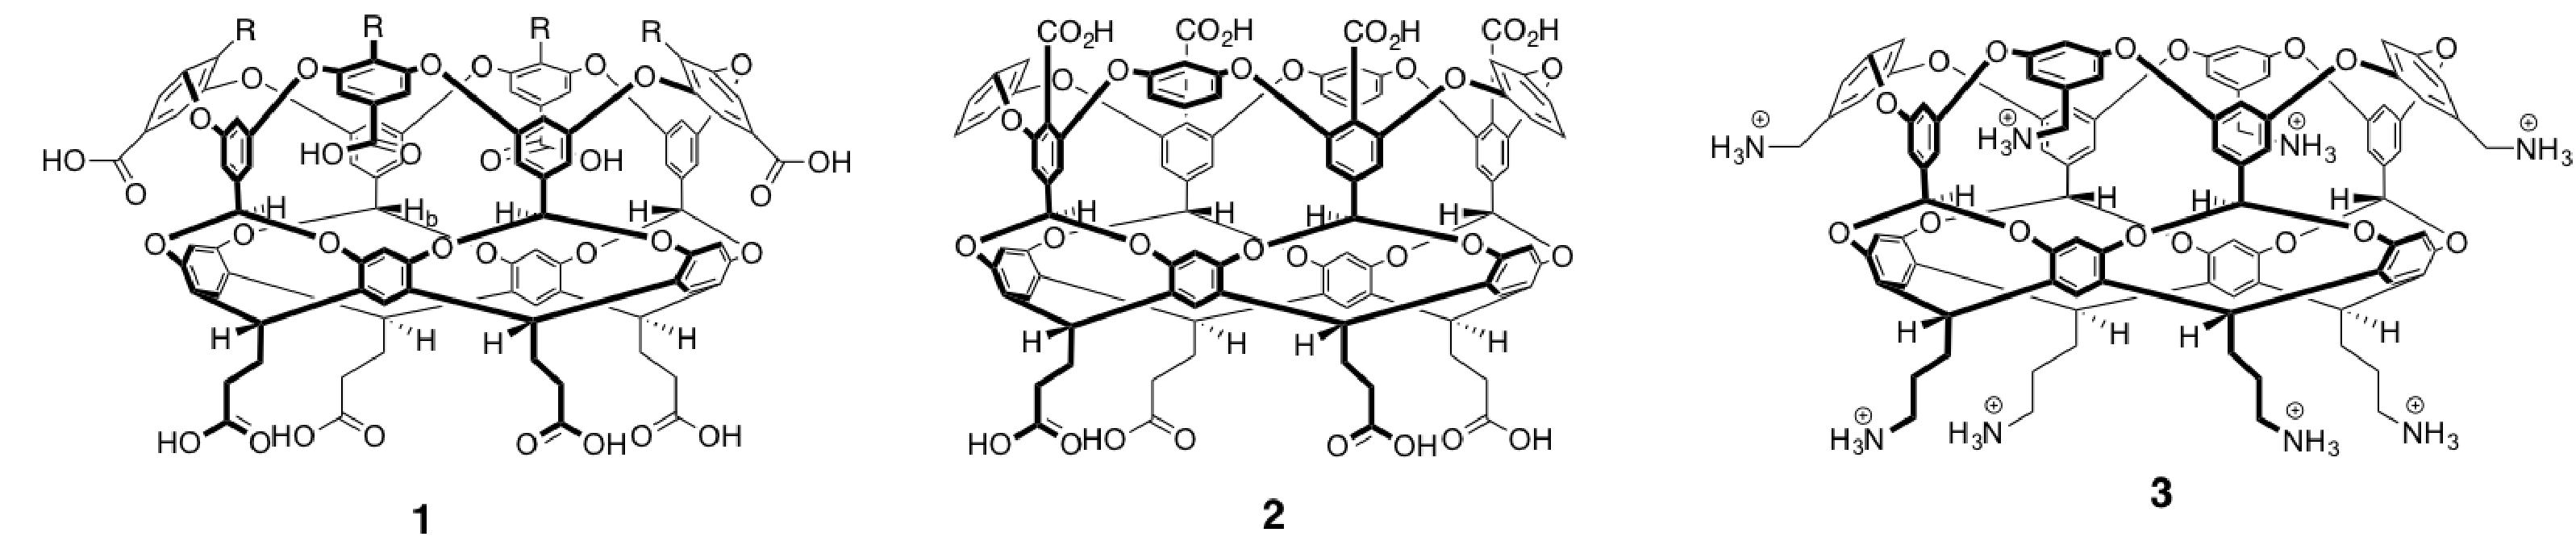
\includegraphics{figures/gdccs.pdf}}

%\end{centering}
\vspace{0.1in}
\caption{\footnotesize {\bf Gibb deep cavity cavitands for SAMPL6-10.}
\label{figure:gdccs}}
\end{centering}
\end{figure}


{\bf Novel deep cavity hosts probe the effects of binding site charge constellations.} 
For future SAMPL challenges, we will expand on the range of hosts by including 2 and 3 in our ITC studies.  
Like cavitand 1, host 2 is an octa-acid derivative.  However, the four benzoate groups are relocated from the extreme exterior in the case of 1, to the rim of the binding pocket in 2.  
We surmise that this will have a direct effect on the binding of charged guests, but more subtly, an indirect effect on guest complexation via changes to the solvation of the empty host.  
Octa-trimethylammonuim cavitand (``positand'' 3) has the same overall architecture as host 1, but inverts the charges on the water solubilizing exterior coat.  While it is not yet clear if this switch in groups relatively remote from the pocket will directly affect guest complexation, results from related systems suggest it can (unpublished).

Guests for the five proposed ITC studies will be obtained from commercial sources, focusing on molecules that probe the limitations of current force-fields as well as new data as it is gathered.   
%JDC asks: "Is it worth noting the guests likely have to be highly soluble?"
% JDC asks whether we should try to pre-calculate guest affinities to aid in selecting those with a large dynamic range or large differences between host variants. I think probably we should propose this -- if we have someone working on SAMPL full-time (Aim 4) this would be very much within what we can do. I'll add something along these lines in edits.

{\bf SAMPL6-10 deep cavity cavitand challenges.} 
The host-guest challenge for SAMPL6 will focus on how well the effect of host carboxylate substituent location can be predicted, and will involve hosts 1 and 2 with a set of five, previously uninvestigated guests.  
SAMPL7 will provide a second iteration of this experiment to test algorithmic improvements in predictive modeling following SAMPL6 by comparing hosts 1 and 3 with a different set of guests.  
We anticipate that because of the relative remoteness of the charged groups in these two hosts, the effects of switching charges will be subtler than the differences between 1 and 2.  
SAMPL8 will consider the effect of common biologically-relevant counterions/salts salts on guest binding, comparing the effects of NaCl and NaI on the complexation of five guests to 1.  
We have previously shown that iodide has a weak affinity for the binding pocket of 1, whilst sodium ions have an affinity for the outer carboxylates~\cite{carnegie_anion_2014}, requiring modeling to capture the differential affinities of these ions in addition to guest affinities to successfully model the observed affinities.  
SAMPL9 will follow up on this by examining the effects of these same two salts on the complexation of five guests to 3, again giving the modeling community time to incorporate algorithmic improvements following SAMPL8. 
While we have not yet quantified salt affinities to host 3, we expect the iodide to have affinity for both the pocket and the positively charged solubilizing groups.  
For SAMPL10 we will consider the effects of co-solvents on the binding of five guests to 1 and 2 to probe the effect of co-solvent competition for the binding site, as well as effects cosolvents may have in weakening the hydrophobic effect. 


%Aim 3 - Generate biologically relevant advanced model systems for protein-ligand binding challenges. (2 pages) 
{\bf Aim 3. Generate biologically relevant advanced model systems for protein-ligand binding challenges.}
We will identify suitable biological protein-ligand model systems (difficult but tractable in order to push the limits of physical techniques) then measure binding and develop these for blind challenges. This will include binding studies on human serum albumin and bromodomains or aspartyl proteases; initial binding data will be expanded by the selection of additional ligands or the creation of mutations in the protein that modulate binding.


%Aim 4 - Coordinate, run, and analyze blind challenges to advance modeling of binding (1.5 pages)
{\bf Aim 4. Coordinate, run, and analyze blind challenges to advance modeling of binding.}
The data collected in Aims 1-3 will drive annual SAMPL blind challenges, allowing the field to test the latest methods and force fields to assess progress, compare them against one another head-to-head, and perform sensitivity analysis to learn how much different factors (protonation state, tautomer selection, solvent model, force field, sampling method, etc.) affect predictive power. Results will then feed back into improved treatment of these factors for subsequent challenges, driving regular cycles of application, learning, and advancement.
%Coordinate and run SAMPL blind challenges
	%Run reference calculations to:
		%a. Test current standard methods/FF
		%b. Facilitate others learning (swap method or FF)
		%c. Do sensitivity analysis (learn what?s important)
		%d. (Give examples of what we?ve learned from this)
		%e. (We will make inputs, outputs, and methods available too)
	%Select and announce null models, run them
	%Do statistical analysis of results (& compare to nulls), report back
	%Work with D3R on meeting coordination
	%Coordinate follow-up experiments as needed (cite examples when this was desirable)
	%Coordinate with JCAMD on special issues
	%Data archival and dissemination
	%   Probably also should comment on archiving/disseminating OLD SAMPL data, which we haven't been able to do (lack of resources)
	%D3R coordination:
	%	a. Co-running workshops with D3R
	%     b. Coordinating challenges with them, submission deadlines offset from D3R challenges



%%%%%%%%%%%%%%%%%%%%%%%%%%%%%%%%%%%%%%%%%%%%%%%%%%%%%%%%%%%%%%%%%%%%%%%%%%%%%%%%%%%%%%%%%%%%%%%%%%%%%%
% TIMELINE
%%%%%%%%%%%%%%%%%%%%%%%%%%%%%%%%%%%%%%%%%%%%%%%%%%%%%%%%%%%%%%%%%%%%%%%%%%%%%%%%%%%%%%%%%%%%%%%%%%%%%%

{\bf \large TIMELINE} %1 page minus a paragraph
%"The timeline is actually likely to be very important here, so I'd strongly suggest we include it, if not expand it to one full page. We have to "sell" the reviewers on how the concept would play out into actual challenges, advances, etc. so that they get a concrete idea of all the good things that will come of this. We should mention when we would hold blind challenges, when data would be released, when meetings would occur, when benchmarks would be published, and what datasets would be generated for the community."



%%%%%%%%%%%%%%%%%%%%%%%%%%%%%%%%%%%%%%%%%%%%%%%%%%%%%%%%%%%%%%%%%%%%%%%%%%%%%%%%
% FIGURE: AIMS OVERVIEW
%%%%%%%%%%%%%%%%%%%%%%%%%%%%%%%%%%%%%%%%%%%%%%%%%%%%%%%%%%%%%%%%%%%%%%%%%%%%%%%%
%\begin{figure}[h]
%\begin{centering}
%\resizebox{\textwidth}{!}{\includegraphics{figures/timeline.pdf}}

%\end{centering}
%\vspace{0.1in}
%\caption{\footnotesize {\bf Timeline.}
%\label{figure:aims-overview}}
%\end{figure}
%%%%%%%%%%%%%%%%%%%%%%%%%%%%%%%%%%%%%%%%%%%%%%%%%%%%%%%%%%%%%%%%%%%%%%%%%%%%%%%%

%%%%%%%%%%%%%%%%%%%%%%%%%%%%%%%%%%%%%%%%%%%%%%%%%%%%%%%%%%%%%%%%%%%%%%%%%%%%%%%%%%%%%%%%%%%%%%%%%%%%%%
% COLLABORATION MANAGEMENT PLAN
%%%%%%%%%%%%%%%%%%%%%%%%%%%%%%%%%%%%%%%%%%%%%%%%%%%%%%%%%%%%%%%%%%%%%%%%%%%%%%%%%%%%%%%%%%%%%%%%%%%%%%

{\large \bf COLLABORATION MANAGEMENT PLAN} % 1 paragraph


{\large \bf OUTLOOK} %or conclusions. 0.5 page


%%%%%%%%%%%%%%%%%%%%%%%%%%%%%%%%%%%%%%%%%%%%%%%%%%%%%%%%%%%%%%%%%%%%%%%%%%%%%%%%%%%%%%%%%%%%%%%%%%%%%%
% BIBLIOGRAPHY
%%%%%%%%%%%%%%%%%%%%%%%%%%%%%%%%%%%%%%%%%%%%%%%%%%%%%%%%%%%%%%%%%%%%%%%%%%%%%%%%%%%%%%%%%%%%%%%%%%%%%%

\eject

%\footnotesize
%\scriptsize
%\bibliographystyle{acm}
\bibliographystyle{nci}
%\bibliographystyle{nar}
\bibliography{sampl-r01}

\end{document}